\chapter{Resultados y análisis}


%Simulación de control
%Pesticida solo
%Corte individual
%Corte Vecinos
%Métodos conjuntos
En este capítulo se describen los resultados encontrados en este trabajo y su interpretación. La cantidad de información arrojada por las ejecuciones del código descritas en el capítulo anterior es amplia, y será analizada a continuación.

\section{Comparación de la dinámica de crecimiento de árboles asintomáticos usando distintos métodos de control}
%Códigos 1, 2 y 3: Gráfica de asintomáticos --------------------------------------------------------------------------------------------------------------------------------COMPARACIÓN DE MÉTODOS
Uno de los intereses de este trabajo ha sido el de observar el comportamiento de los métodos usados en el campo mexicano para reducir la propagación de la enfermedad. Los métodos de especial interés son la reducción directa y periódica de la población de psílidos, y la eliminación de los árboles con síntomas. A continuación, se muestra la evolución temporal de las poblaciones en una huerta en condiciones normales\cite{dala2019effect} \cite{robles2012protocolo}.
\begin{figure}[H]
\centering
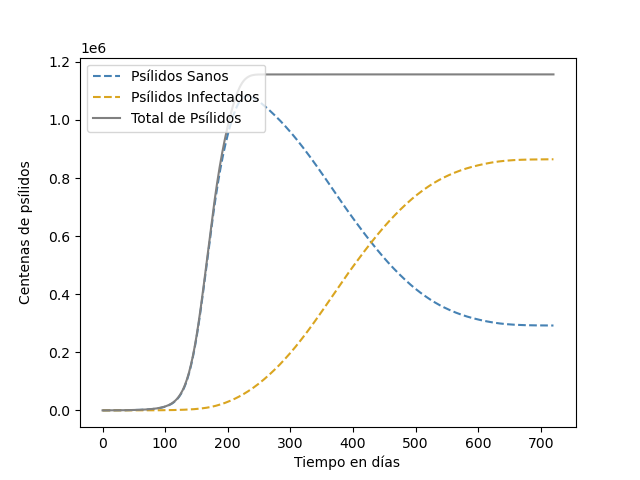
\includegraphics[width=0.7\textwidth,keepaspectratio=true]{images/Imágenes C6/C6-0.png}
\caption{Crecimiento de las poblaciones de psílidos infecciosos, sanos y totales en un campo sin ningún método de control.}
\end{figure}
%Hechos:
%PRIMERO: La aplicación de pesticidas es la mejor herramienta para combatir la enfermedad si no se tiene acceso a información sobre árboles asintomáticos, es buena incluso sin el corte de los árboles
La primera observación que se ha desprendido de las simulaciones en las que se compararon los métodos de control, es que la aplicación de pesticidas o algún agente que reduzca en general a la población, es la mejor herramienta para combatir el crecimiento de la enfermedad dentro de la huerta. Especialmente si no se tiene acceso a ninguna clase de información sobre la cantidad y ubicación de los árboles asintomáticos y los infectados, llegando a ser buena incluso sin el corte de los árboles sintomáticos. A continuación, se muestran tres gráficas distintas que representan a la matriz de posiciones, cada una generada por la ejecución del código con distintos métodos de control.
\begin{figure}[H]
\centering
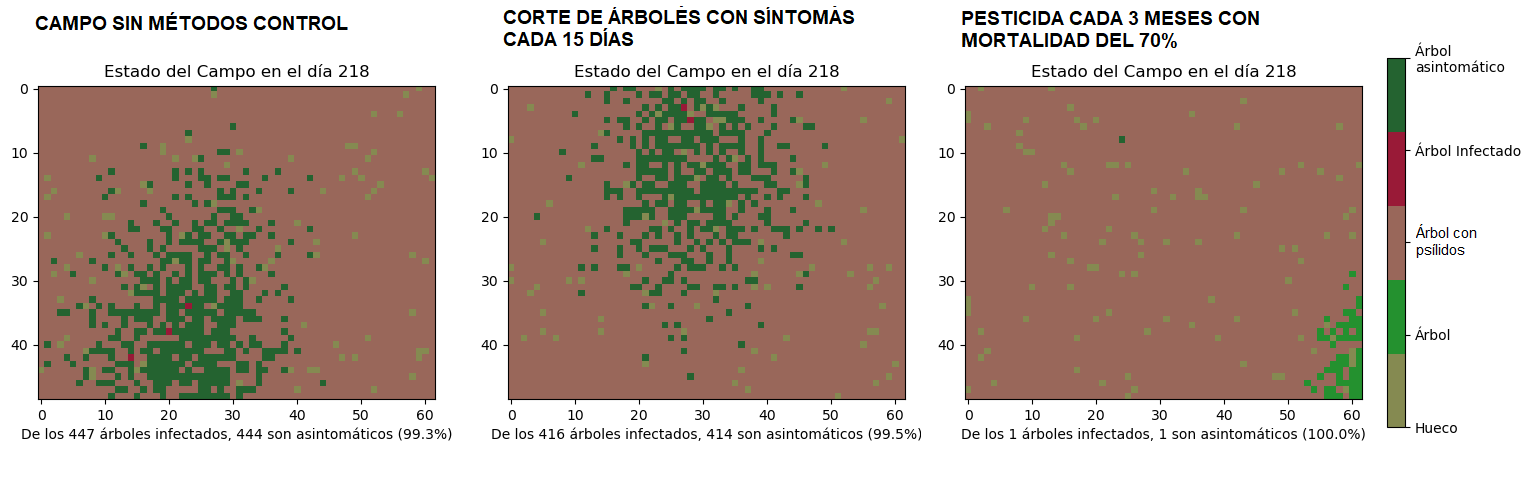
\includegraphics[width=1\textwidth,keepaspectratio=true]{images/Imágenes C6/C6-1.png}
\caption{Comparación del estado tres campos con distintos métodos de control luego de 218 días de haber sido inoculado con psílidos infecciosos}
\end{figure}
De lo anterior, se puede observar la importancia que tiene la aplicación de pesticidas de forma periódica y su contraste con métodos que prescinden de ella. Como se puede observar, cuando las medidas de control son endebles, la propagación asintomática es veloz, y mientras que para el momento en el que las huertas con control pesticida comienzan a infectarse, en las huertas sin pesticidas la infección ya tiene un avance significativo. También se puede observar que la tala de los árboles sintomáticos aporta algo de control a propagación, pero este esfuerzo es insuficiente. 

%SEGUNDO; La acción combinada de los anteriores métodos retrasó en promedio la aparición de árboles sintomáticos hasta los 260 días

Otra faceta explorada en este trabajo es la del control conjunto y coordinado de los dos métodos anteriores, en ella se encontró que su acción combinada retrasó la aparición de árboles sintomáticos hasta los 260 días en promedio. Y quedó en evidencia el resultado predecible de que cuanto más campañas de aplicación de pesticidas haya, menos se esparce la bacteria a través de los árboles de la huerta. A continuación, se muestran dos campos en los que el período de revisión de síntomas es de quince días y el periodo de aplicación de pesticidas es de dos meses y quince días respectivamente, representando este último un caso extremo. Cada campo es mostrado en el día en el que han aparecido los primeros árboles con síntomas.
\begin{figure}[H]
\centering
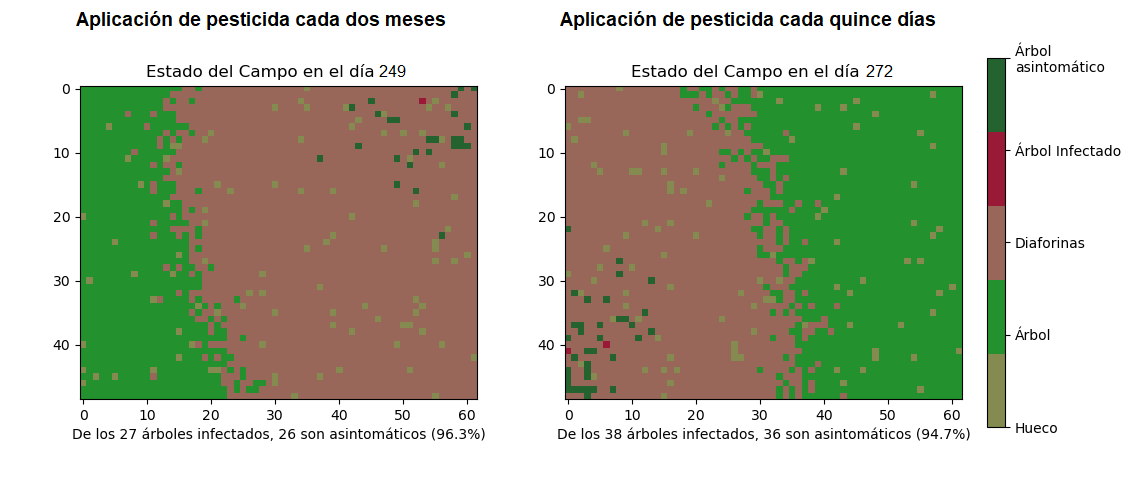
\includegraphics[width=1\textwidth,keepaspectratio=true]{images/Imágenes C6/C6-2.png}
\caption{Comparación del estado dos campos en los que se aplica pesticida con diferentes períodos, luego de 218 días.}
\end{figure}

%TERCERO: Aunque los métodos combinados, no redujeron a cero la población de psílidos, tuvieron un impacto mayor en la población de psílidos infecciosos y esto parece tener implicaciones directas en la cantidad de árboles infectados

De lo anterior, queda claro que aunque este método de control reduce notablemente la población de psílidos, no la elimina del todo, sin embargo esto no evita que tenga un impacto considerable en la población de psílidos infecciosos. Se ha visto recurrentemente en las simulaciones de este trabajo que hay una fuerte relación entre las regiones con gran presencia de árboles infectados y las regiones con gran presencia de psílidos infecciosos, de tal forma que en la mayoría de los casos, estas regiones suelen ser casi idénticas, y esto parece tener implicaciones directas en la cantidad de árboles infectados, y esto podría ser un indicio de que tener datos fiables de la distribución y cantidad de psílidos infecciosos en una huerta, conduciría irremisiblemente a estar en condiciones de inferir la región de árboles asintomáticos.

%CUARTO: El efecto de cortar los árboles vecinos es despreciable
En esta simulación, también se valoró la viabilidad de talar a los árboles vecinos de un árbol detectado como infectado, sin embargo su impacto en la reducción de la enfermedad fue despreciable, y su repercusión en la reducción de la cantidad de árboles de la huerta fue grande.
	
%Conclusión: 
En síntesis, la efectividad de los métodos estudiados se ha puesto de manifiesto, además de la evidencia de que estos métodos conjuntos son aún más efectivos. También se ha visto que el problema de combatir la propagación de HLB se puede ceñir de buena forma al combate exclusivo de los psílidos infecciosos, de modo que conocer la distribución de estos dentro de la huerta es una herramienta útil para inferir la distribución de árboles asintomáticos dentro de ella.


%Códigos 1, 3, 4, 5 y 6: Gráfica de Distribución de psílidos y gráfica de distribución de asintomáticos ---------------------------------------------------------------------DINÁMICA DE LOS PSÍLIDOS INFECCIOSOS
\section{Dinámica de los psílidos infecciosos}
%Hechos: 
%PRIMERO: La distribución de psílidos infecciosos y sanos no es igual, pese a que sus patrones de movimiento son iguales, los árboles infectados son los que alojan a la gran mayoría de psílidos ifectados. 
Uno de los principales resultados, respecto a la dinámica de los psílidos, ha sido que la distribución de psílidos infecciosos no es igual a la de los sanos pese a que sus reglas de movimiento son iguales dentro del código de la simulación, y en todas las simulaciones se ha observado que los árboles infectados son los que alojan a la gran mayoría de psílidos infecciosos, como se ha dicho antes. A continuación, en la Figura 5.4, se muestran las distribuciones de psílidos dentro de una huerta. El primer cuadro corresponde a la \textit{matriz de posiciones} y los tres restantes corresponden a los \textit{campos de psílidos} descritos en el capítulo 4, se ha tomado el día 134 porque en él se ha notado el mayor contraste.
\begin{figure}[H]
\centering
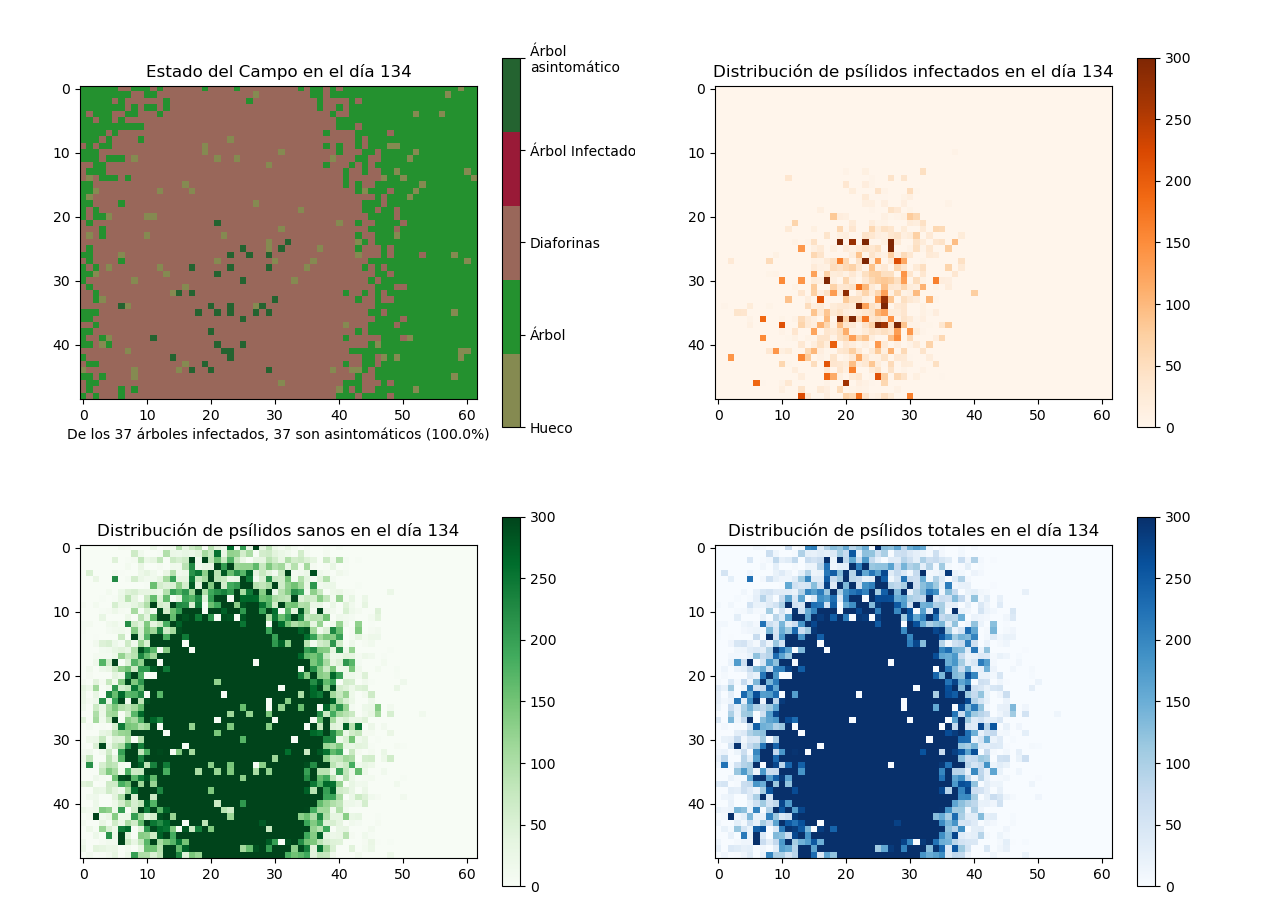
\includegraphics[width=1.\textwidth,keepaspectratio=true]{images/Imágenes C6/C6-3.png}
\caption{Estado del un campo sin control luego de 134 días de haber sido inoculado con psílidos infecciosos. }
\end{figure}
En la figura anterior, el cuadro superior izquierdo muestra la distribución de árboles asintomáticos y sanos, el resto de cuadros muestran la concentración de psílidos clasificados, en ella puede observar que la distribución de los psílidos sanos prácticamente se ajusta a la de los psílidos totales en el campo, esto se puede ver como que las zonas con presencia de psílidos tienen por lo general al menos algo de presencia de psílidos sanos, sin embargo, esto no sucede igual con los psílidos infecciosos, que están por lo general en las mismas zonas donde hay presencia de árboles infectados, ya sean estos asintomáticos o no.
La figura anterior muestra una huerta sin ningún método de control, pero todas las huertas simuladas tienen esta característica, además de que tienden a la eventual infección de todos sus árboles y a ser ocupadas por psílidos infecciosos. El crecimiento de las regiones de psílidos infecciosos sigue al crecimiento del total de psílidos.

%SEGUNDO: Hay incluso algunos huertos, donde la infección es tan fuerte, que en los lugares con psílidos infecciosos hay gran ausencia de psílidos sanos.
Se ha observado también que cuando la infección es suficientemente fuerte en algún huerto, en las zonas con psílidos infecciosos hay una gran ausencia de psílidos sanos. La explicación que se propone es que esto es una consecuencia de que la zona y su entorno han alcanzado el máximo de población de psílidos que puede alojar, de modo que los psílidos difícilmente emigran y la población no se renueva, y esto, sumado al largo tiempo en el que el árbol ha sido transmisor de la bacteria, provoca que la mayoría de psílidos dejen de ser sanos para convertirse en infecciosos. Esta propuesta es congruente con el hecho observado de que los psílidos que emergen de los huevecillos depositados en árboles infectados, suelen portar concentraciones más altas de la bacteria, y así, los psílidos sanos terminan por morir o por infectarse.
Este efecto podría ser también una forma de detectar indirectamente las zonas con mayor presencia y longevidad de árboles infectados; se podrá deducir que cuanto menor sea la fracción de psílidos sanos en alguna zona, la enfermedad en esa zona es más intensa. Esto tiene la evidente ventaja de que la medición se convierte en un asunto de proporción y no de cantidad, siendo esta una vía más factible para los agricultores. Si se toma una muestra de cierta cantidad representativa de los psílidos que habitan un punto de la huerta, y se cuenta la cantidad de psílidos sanos, se estaría en condiciones de estimar la intensidad de la enfermedad en ese punto. Este efecto se ilustra a continuación, en la figura 5.5:
\begin{figure}[H]
\centering
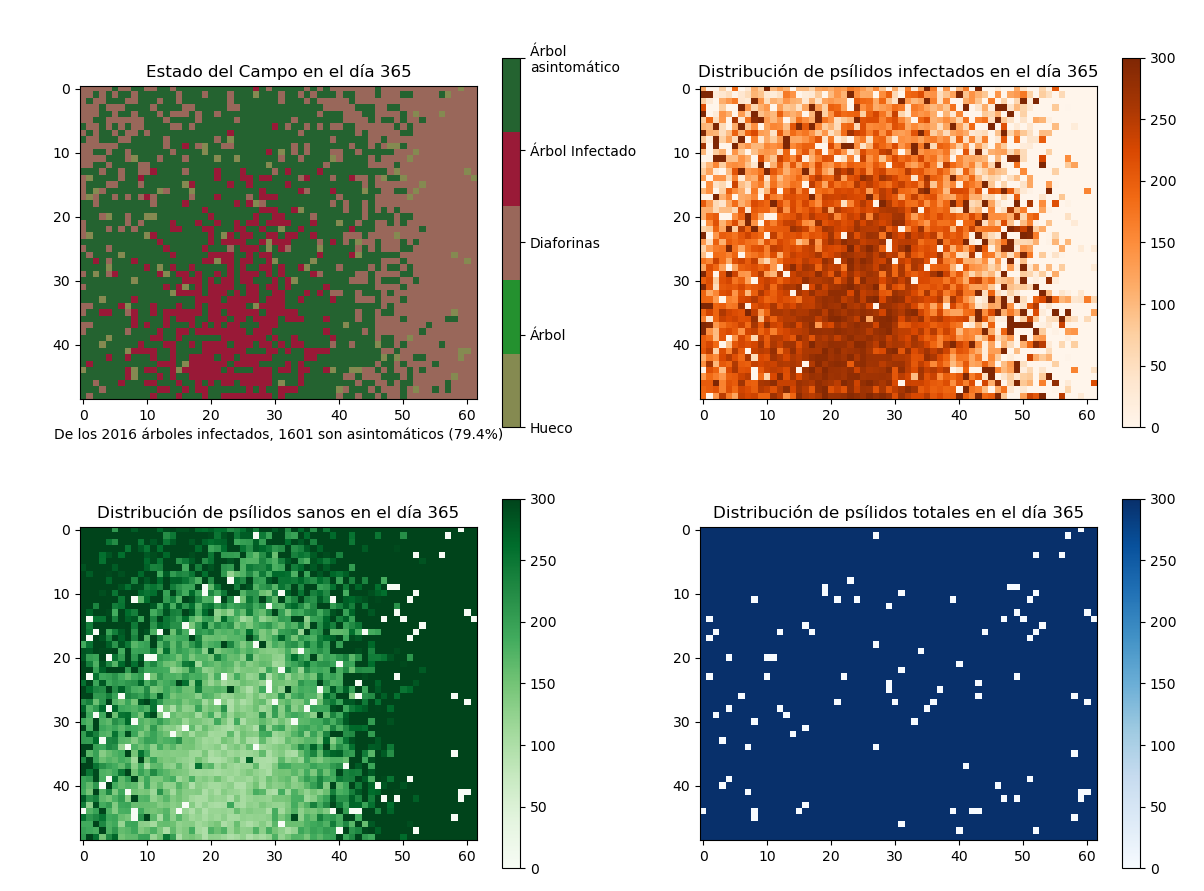
\includegraphics[width=1.\textwidth,keepaspectratio=true]{images/Imágenes C6/C6-4.png}
\caption{Estado del un campo sin control luego de un año. La ausencia de psílidos sanos es notable en las zonas con más árboles sintomáticos.}
\end{figure}

%TERCERO: La distribución de población de psílidos infecciosos es una mancha
Algo que se aprecia en todos los mapas de distribución de los psílidos, sin importar incluso si se usan métodos de control, es que suelen ser manchas ligeramente ovaladas verticalmente, con un centro normalmente cercano al lugar donde los psílidos fueron inicialmente depositados, y cuyo radio crece a través del tiempo. Este hecho implica que la zona de riesgo de contagio está acotada por alguna distancia que dependa del tiempo transcurrido. Sería de interés para estudios futuros el investigar la relación que existe entre la proporción de psílidos infecciosos en alguna zona, y el radio de la zona de psílidos infecciosos.

%CUARTO:La población de psílidos forma además una especie de onda 
La última observación de interés en cuanto a la dinámica de los psílidos infecciosos es la presencia de un «patrón de ondas» generado en las huertas en las que hubo aplicación de pesticidas periódicamente. Hasta ahora no se tiene ninguna hipótesis a este respecto, un ejemplo se muestra a continuación, en la figura 5.6:
\begin{figure}[H]
\centering
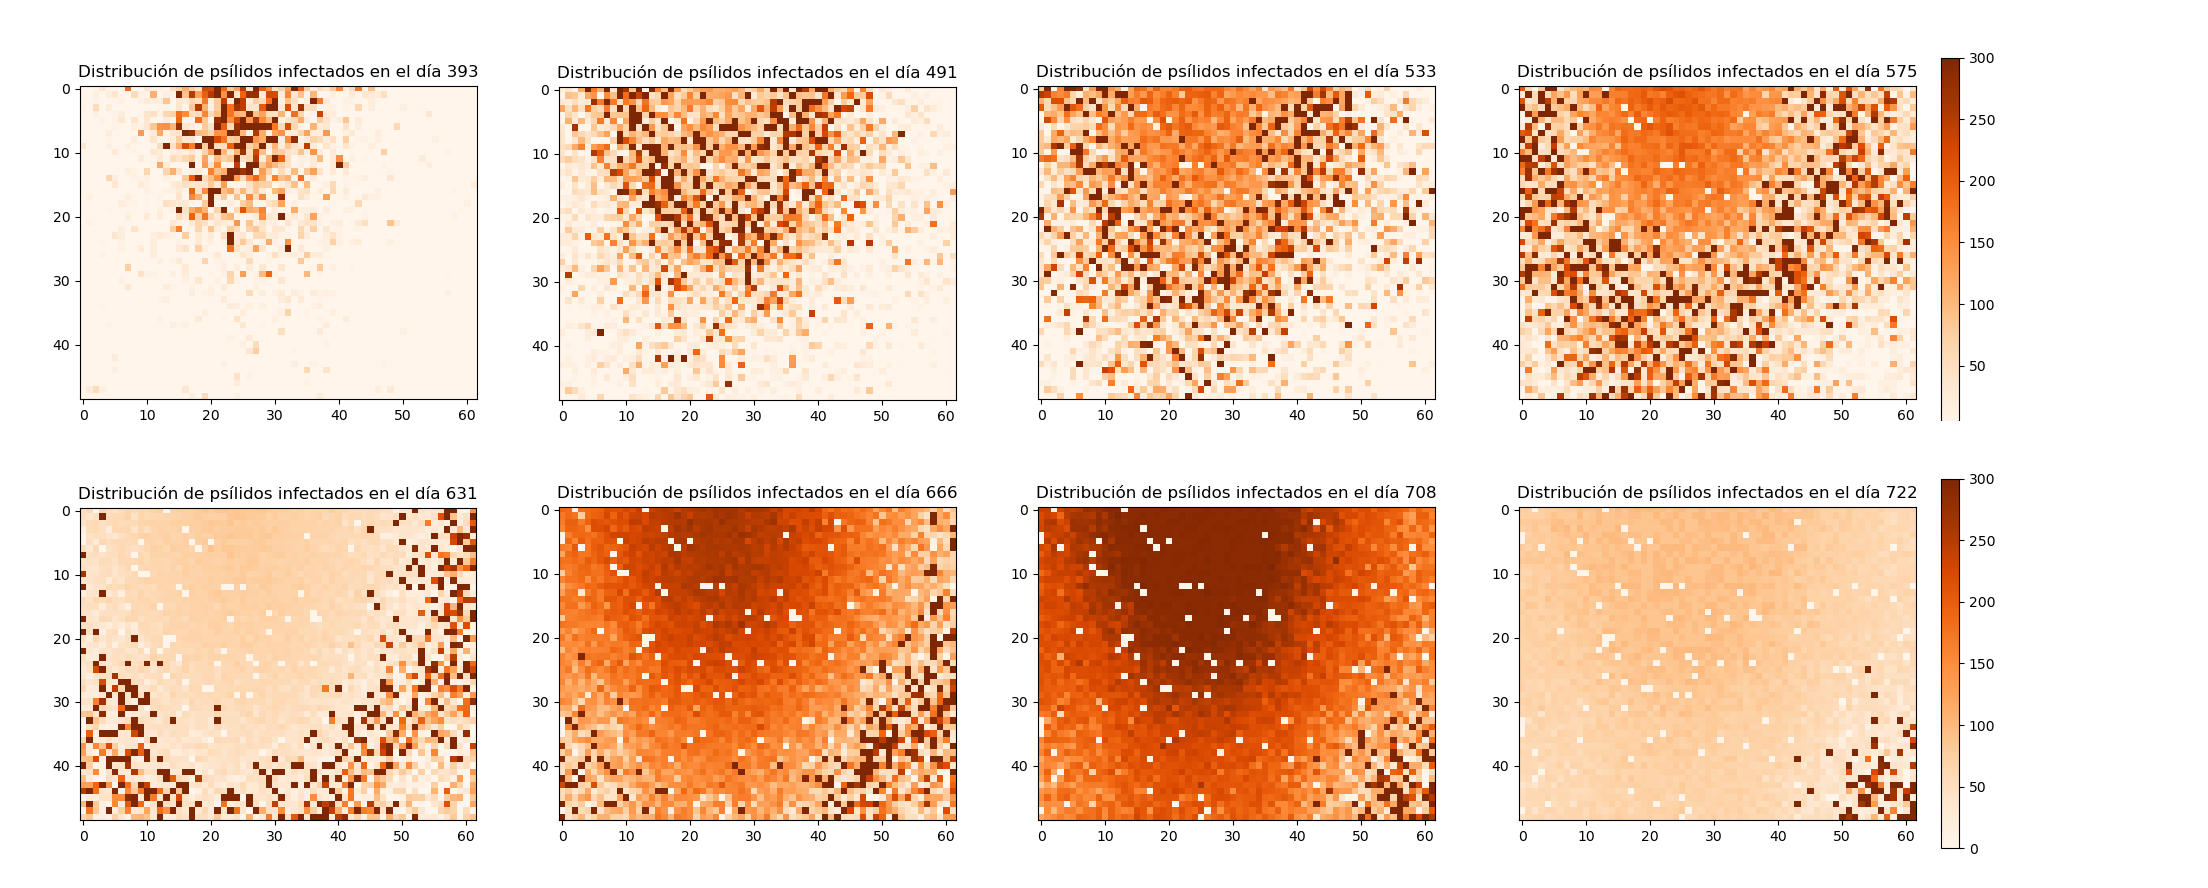
\includegraphics[width=1.05\textwidth,keepaspectratio=true]{images/Imágenes C6/C6-5.png}
\caption{Patrón formado por el crecimiento y distribución de la población de psílidos infecciosos con el pasar de los días.}
\end{figure}


%Códigos todos -------------------------------------------------------------------------------------------------------------------------------------------------------------VIABILIDAD DEL MÉTODO DE MEDICIÓN EN T SOBRE OTROS MÉTODOS
\section{Justificación del \textit{Método en «T»}}

%Hechos:
%ÚNICO:En todas las simulaciones con todas las variables, los psílidos, los asintomáticos, y los sintomáticos son manchas crecientes. Y más aún, los primeros sintomáticos suelen ser el centro de los asintomáticos.
Hasta ahora, no se ha hablado de la relación que tienen las manchas de crecimiento de los distintos tipos de agentes que conforman el sistema. En esta sección se abordará dicha dinámica y se la relacionará con el método de vigilancia propuesto por el protocolo oficial para detectar árboles asintomáticos. Se ha observado en todas las simulaciones que se hicieron, sin importar qué variables se modificaran, ni cómo se modificaran, que los agentes del campo se expanden formando manchas crecientes y concéntricas.
Las primeras apariciones puntuales son las que resultan de la colocación inicial de psílidos, tanto psílidos sanos como infecciosos, estos puntos con psílidos comienzan a convertirse de a poco en una mancha que crece alrededor del lugar donde fueron colocados al principio, este lugar se convierte normalmente en centro de la mancha de psílidos y de todas las que le sucederán. Cuando ha pasado suficiente tiempo, la mancha de psílidos es suficientemente grande y son observadas las primeras apariciones puntuales de árboles asintomáticos en el centro de la mancha de psílidos, y replicando a su antecesora, esta mancha de árboles asintomáticos también comienza a expandirse de a poco, esto mientras la mancha de psílidos totales sigue creciendo. Después de que la mancha de los árboles asintomáticos ha cobrado cierto tamaño, y en el caso de esta simulación, en torno a los 200 días, los primeros brotes puntuales de árboles sintomáticos aparecen, replicando en su crecimiento a las manchas que lo antecedieron. Además, si se hace una distinción entre la mancha de psílidos infecciosos y la de psílidos totales, se puede observar un comportamiento similar.
Lo anterior da como consecuencia que los primeros árboles que presentan síntomas en una huerta suelen ser el centro de la infección, y ese centro es el lugar de arribo de los psílidos y también el lugar a partir del cual los árboles asintomáticos han comenzado a infectarse. A continuación, en la Figura 5.7, se ilustran estas tres fases.
\begin{figure}[H]
\centering
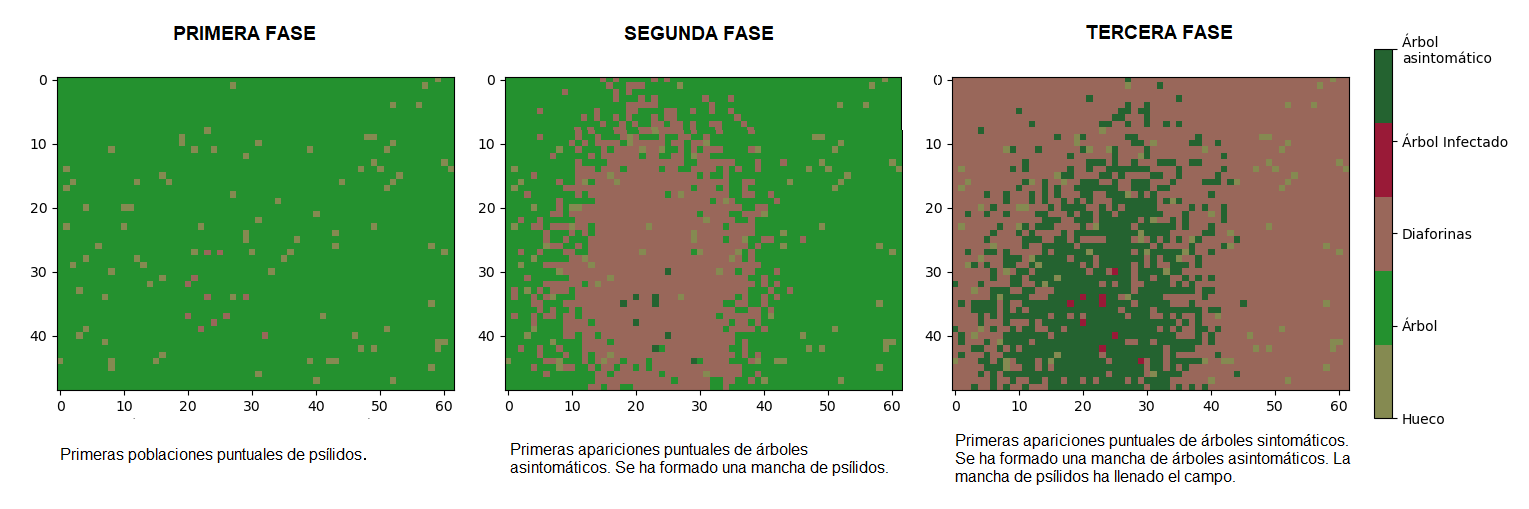
\includegraphics[width=1.05\textwidth,keepaspectratio=true]{images/Imágenes C6/C6-6.png}
\caption{Crecimiento concéntrico de la distribución de psílidos, árboles infectados, y árboles sintomáticos.}
\end{figure}

%Ideas:
Dado que la evidencia consultada indica que los psílidos que llegan a los huertos suelen instalarse en los árboles de los bordes, o cerca de ellos, el método de «revisión en T» del que se habló en el capítulo 3, queda respaldado. Si los psílidos arriban por los bordes y su población crece en manchas, y a estas manchas de psílidos seguirán las manchas de árboles asintomáticos, entonces, los árboles asintomáticos se propagarán también en manchas desde los bordes, y la estrategia de revisión «en T» se ajusta bien a esta característica.
Más aún, se puede establecer que, en general, cuando se detecta un árbol con síntomas, hay una buena probabilidad de que este esté en el centro de la mancha de árboles asintomáticos. Por esta razón sería de interés el calibrar esta simulación en virtud de estar en condiciones de estimar el tamaño de estas manchas asintomáticas en función del tiempo en las huertas reales.
%Propuestas:
Con esta información, se puede asegurar que una buena forma de buscar árboles asintomáticos a partir de la detección de un árbol con síntomas es mediante el método «en T» cuando el árbol esté cerca a los bordes, y en general, si el árbol se encontrase al centro de la huerta, podría extenderse el patrón, de ser una te a ser una cruz como se ve en la figura siguiente (5.8):
\begin{figure}[H]
\centering
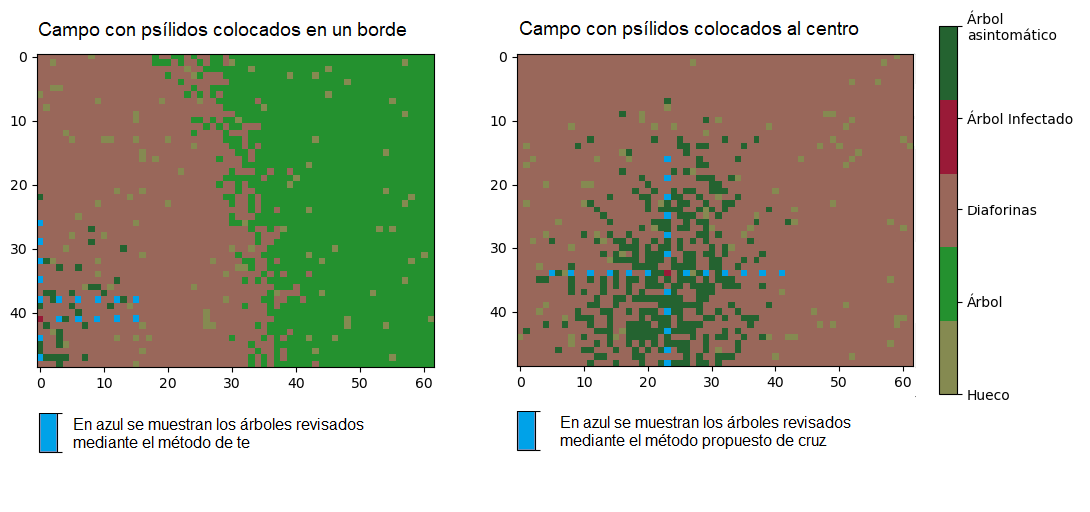
\includegraphics[width=1.05\textwidth,keepaspectratio=true]{images/Imágenes C6/C6-7.png}
\caption{A la izquierda, ilustración del «método en T» descrito en el capítulo tercero. A la derecha, un método propuesto para revisar orígenes de infección al centro.}
\end{figure}
	
%Códigos algunos xd--------------------------------------------------------------------------------------------------------------------------------------------------------LA RELACIÓN ENTRE LOS ASINTOMÁTICOS Y LOS SINTOMÁTICOS
\section{La relación entre árboles asintomáticos y sintomáticos}
%Hechos:
%SEGUNDO: Del mismo modo las gráficas de crecimiento de árboles sintomáticos e infectados son similares salvo un desfase de 200 días, ver árboles Control día 722 -
La primera observación respecto a la relación que existe entre el crecimiento de los árboles asintomáticos y los sintomáticos tiene que ver con el comportamiento descrito anteriormente, en el que la expansión de las manchas de árboles con síntomas sigue a la expansión de los árboles asintomáticos. Este efecto queda de manifiesto cuando se analiza la gráfica del crecimiento de árboles asintomáticos y con síntomas de un huerto sin ningún método de control. El crecimiento de la población de árboles sintomáticos obedece al crecimiento de la población de psílidos, como se ve en la Figura 5.9.
\begin{figure}[H]
\centering
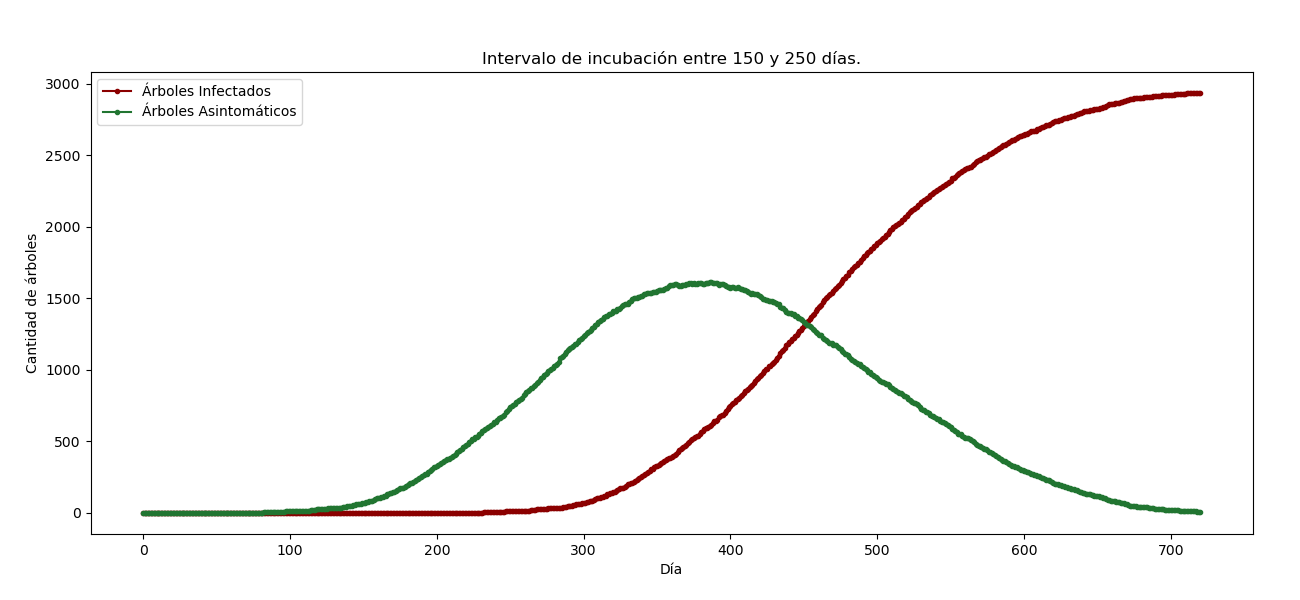
\includegraphics[width=1\textwidth,keepaspectratio=true]{images/Imágenes C6/C6-8.png}
\caption{Gráfica de la cantidad de árboles infectados y sanos, respectivamente, a través del tiempo, para una huerta sin control.}
\end{figure}
%HECHO TERCERO: La gráfica verde es la derivada de la roja desplazada, incluso cuando se aplica el corte
La línea verde está estrechamente relacionada con la trayectoria de la línea roja, esto es que el crecimiento en la población de árboles asintomáticos puede ser asociado con el crecimiento de la población de árboles sintomáticos. El crecimiento de la población del psílido está modelado como una función logística, y la gráfica de los árboles sintomáticos tiene un comportamiento similar al de la gráfica de una función logística. La línea verde de árboles asintomáticos tiene una silueta parecida a la de la distribución logística, la función de densidad de probabilidad cuya función de distribución es justamente la función de distribución logística.

%Idea:
El crecimiento en los árboles sintomáticos puede explicarse mediante el hecho de que, en el modelo, la probabilidad de que un árbol se infecte está solamente dada por la cantidad de psílidos infecciosos que aloje, algo que tiene como consecuencia que la cantidad de psílidos que haya en la huerta, en algún momento, condicionará la cantidad de árboles que se infecten en ese momento, de modo que es por esta razón que el crecimiento de las infecciones en una huerta es una calca del crecimiento de los psílidos infectados en esa misma huerta.
Una línea para continuar la investigación, podría ser la búsqueda de alguna forma analítica de estimar la cantidad de árboles asintomáticos dados los datos de la cantidad de árboles con síntomas.

La relación entre ambas poblaciones de árboles parece estar presente incluso cuando se aplican métodos de control como el pesticida y el corte de árboles sintomáticos. Cuando el pesticida es aplicado, las curvas se aplanan más o menos en función de la intensidad de la aplicación del pesticida, mientras que al hacer uso del corte de árboles sintomáticos, el comportamiento se mantiene a pesar de las reducciones en la población de árboles infectados; a continuación se muestra la gráfica de poblaciones de árboles de una huerta en la que fue aplicado el método de tala.
\begin{figure}[H]
\centering
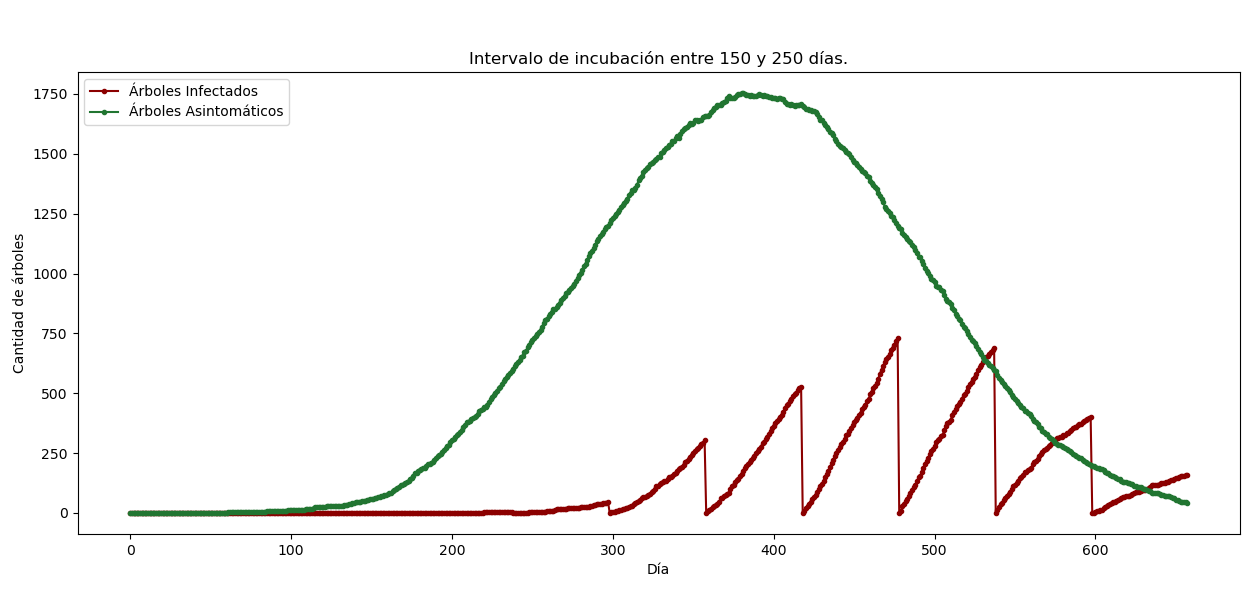
\includegraphics[width=1\textwidth,keepaspectratio=true]{images/Imágenes C6/C6-9.png}
\caption{Gráfica de la cantidad de árboles infectados y sanos, respectivamente, a través del tiempo, para una huerta con eliminación de árboles con síntomas.}
\end{figure}
Este comportamiento implica que de desarrollar una herramienta analítica capaz de estimar la cantidad de árboles asintomáticos en función de la cantidad de árboles sintomáticos, aún en distintos escenarios de control, ésta conservaría tal poder.


%Idea: En lugar de la derivada, graficar asintomáticos vs sintomáticos y dar la curva